% 原书 p.204–p.213（PDF p.212–p.221）
% 第 8 章 8.3 节：稳定映射（Stable Map）
% 说明：8.4 节自 p.222 开始，见 ch08-s04.tex；本节 p.212 上部仍属 8.2 节（见 ch08-s02.tex）。

\section{稳定映射（Stable Map）}
% >>> p212

\begin{keytakeaways}
\begin{itemize}
  \item 几何图像：$J$-全纯曲线的模空间\textbf{不紧}——一族曲线可以「冒泡」成一个树状构型（若干
        $S^2$ 在结点处相粘），或在覆盖意义下退化为多重覆盖曲线；稳定映射正是把极限对象也纳入
        计数框架的紧化工具。
  \item 数学工具：Riemann--Hurwitz 公式 (8.19)、(8.20) 的覆盖次数关系；多重覆盖与单的
        （simple）曲线（定义 8.3.1--8.3.2）；带 $k$ 个标记点的树状稳定映射（定义 8.3.3）；
        四个模空间 $\mathcal{M}^*_k$、$\mathcal{M}_k$ 及其紧化 $\overline{\mathcal{M}^*_k}$、
        $\overline{\mathcal{M}_k}$。
  \item 本节结论：Gromov 定理 8.3.2——在 Gromov 序列拓扑下
        $\overline{\mathcal{M}_k(A,J)}$ 紧，且 $\mathcal{M}^*_k(A,J)$ 是其中的开稠子集，对通有
        $\omega$-相容 $J$ 还是（实）维数 $=\dim_\R M+2c_1(TM)(A)+2k-6$ 的流形（式 (8.27)、
        (8.28)）；由此得到分层结构 (8.29)。
  \item 阅读要点：稳定性条件 (iii) 只对常值 $S^2$-分支提出要求；计数时真正要数的是「模去
        重新参数化的类」而非曲线本身（PSL(2,$\C$) 作用，见 (8.22)--(8.24)）。
\end{itemize}
\end{keytakeaways}

本节转回 $J$-全纯曲线的研究——把曲线看作从亏格为零的 Riemann 曲面 $(S^2,j)$ 到近复流形
$(M,J)$ 的映射。映射作为函数的推广，其行为可能相当复杂。本节将说明研究（一族）$J$-全纯曲线时
可能遇到的问题，引入稳定映射的概念，并考察这类曲线的模空间。

\textbf{$J$-全纯曲线的极限。} 研究曲线/映射族的性态时，一个自然的焦点是它的极限。研究极限
已成为几何与拓扑中许多分支的中心课题。然而自然界有一个不幸的事实：$J$-全纯曲线序列可能收敛到
一个奇怪的极限！下面是一个例子。

\begin{wexam}{8.3.1}（[229] 中的例 8.17）
  设 $u_n\colon(S^2,j)\to(\CP^2,J_{\mathrm{std}})$ 是一列 $J$-全纯曲线，其中
  $J_{\mathrm{std}}$ 是 $\CP^2$ 上的标准复结构，而 $u_n$ 定义为
  \begin{equation}\tag{8.15}
    [z_0:z_1]\mapsto\Bigl[z_0^2:\frac{z_1^2}{n}:z_0z_1\Bigr]
  \end{equation}
  （这里把 $S^2$ 与 $\CP^1$ 等同）。若记 $[z_0^2:z_1^2/n:z_0z_1]=[X:Y:Z]\in\CP^2$，则
  (8.15) 定义的 $u_n$ 的像等于
  \[
    \operatorname{im}(u_n)
      =\Bigl\{[X:Y:Z]\in\CP^2\ \Big|\ XY=\frac{Z^2}{n}\Bigr\}.
  \]
  特别地，当 $n\to\infty$ 时，极限曲线由 $XY=0$ 描述（于是 $X=0$ 或 $Y=0$）。因此
  \[
    \operatorname{im}(u_\infty)=\{[0:Y:Z]\}\cup\{[X:0:Z]\}=:A_0\cup A_1.
  \]
  \hfill$\square$
\end{wexam}

这里，$A_0$ 与 $A_1$ 构成 $\CP^2$ 中两份 $\CP^1$，它们在单点 $[0:0:1]$ 处相连。下面是一个朴素的
问题。

% >>> p213
\begin{wque}{8.3.1}
  对标准近复结构 $J_{\mathrm{std}}$，极限 $\operatorname{im}(u_\infty)$ 是否可能是某条
  $J_{\mathrm{std}}$-全纯球面的像？换言之，是否存在
  $u\colon(\CP^1,j)\to(\CP^2,J_{\mathrm{std}})$ 使得
  $\operatorname{im}(u)=\operatorname{im}(u_\infty)$？
\end{wque}

为回答这个问题，让我们更仔细地考察收敛 $u_n\to u_\infty$。一方面，就 (8.15) 中的表达式而言，
对点 $[z_0:z_1]\in\CP^1$，极限是 $u_\infty([z_0:z_1])=[z_0^2:0:z_0z_1]$。注意
$u_\infty([z_0:z_1])$ 只在 $z_0\ne0$ 时良定义，而此时
\begin{equation}\tag{8.16}
  u_\infty([z_0:z_1])=[z_0:0:z_1]\cong\CP^1\setminus\{[0:1]\}.
\end{equation}
这表明可以考虑如下 $J_{\mathrm{std}}$-全纯映射
\begin{equation}\tag{8.17}
  u\colon\CP^1\to\CP^2\quad\text{定义为}\quad[z_0:z_1]\mapsto[z_0:0:z_1],
\end{equation}
它覆盖了 $\operatorname{im}(u_\infty)$ 的几乎处处，唯独漏掉定义域 $\CP^1$ 中点 $[0:1]$ 的像。
另一方面，出于好奇，让我们沿 $u_n$（当 $n\to\infty$）或沿 (8.17) 定义的 $u$ 追踪点 $[0:1]$。
由于对任意 $n\in\N$ 都有 $u_n([0:1])=[0:1/n:0]=[0:1:0]$，这个点在该收敛过程中是稳定的。同时，
由 (8.17) 有 $u([0:1])=[0:0:1]$。由于 $[0:1:0]\ne[0:0:1]$，(8.17) 中尝试的映射 $u$ 并不是
问题 8.3.1 中所要求的映射。

事实上，与前面得到的 $\operatorname{im}(u_\infty)=A_0\cup A_1$ 相比，$u$ 的像只覆盖了 $A_1$，
而整个 $A_0$（更确切地说 $A_0\setminus\{[0:0:1]\}$）被遗漏了。这个 $A_0$ 称为
$J_{\mathrm{std}}$-全纯曲线 $u_n$ 收敛过程中的一个\textbf{冒泡}（bubbling）。下面的练习表明：
也可以通过考虑 $J_{\mathrm{std}}$-全纯曲线
$v\colon(\CP^1,j)\to(\CP^2,J_{\mathrm{std}})$ 来恢复 $A_0$，但不幸的是，与上面的 $u$ 相对称，
这个映射 $v$ 会遗漏分支 $A_1$。因此，为恢复整个 $\operatorname{im}(u_\infty)$，人们自然会考虑
「并映射」$(u,v)$，其定义域是两份 $\CP^1$ 在点 $[0:1]$ 处相粘（见图 8.1）。

\begin{figure}[htbp]
  \centering
  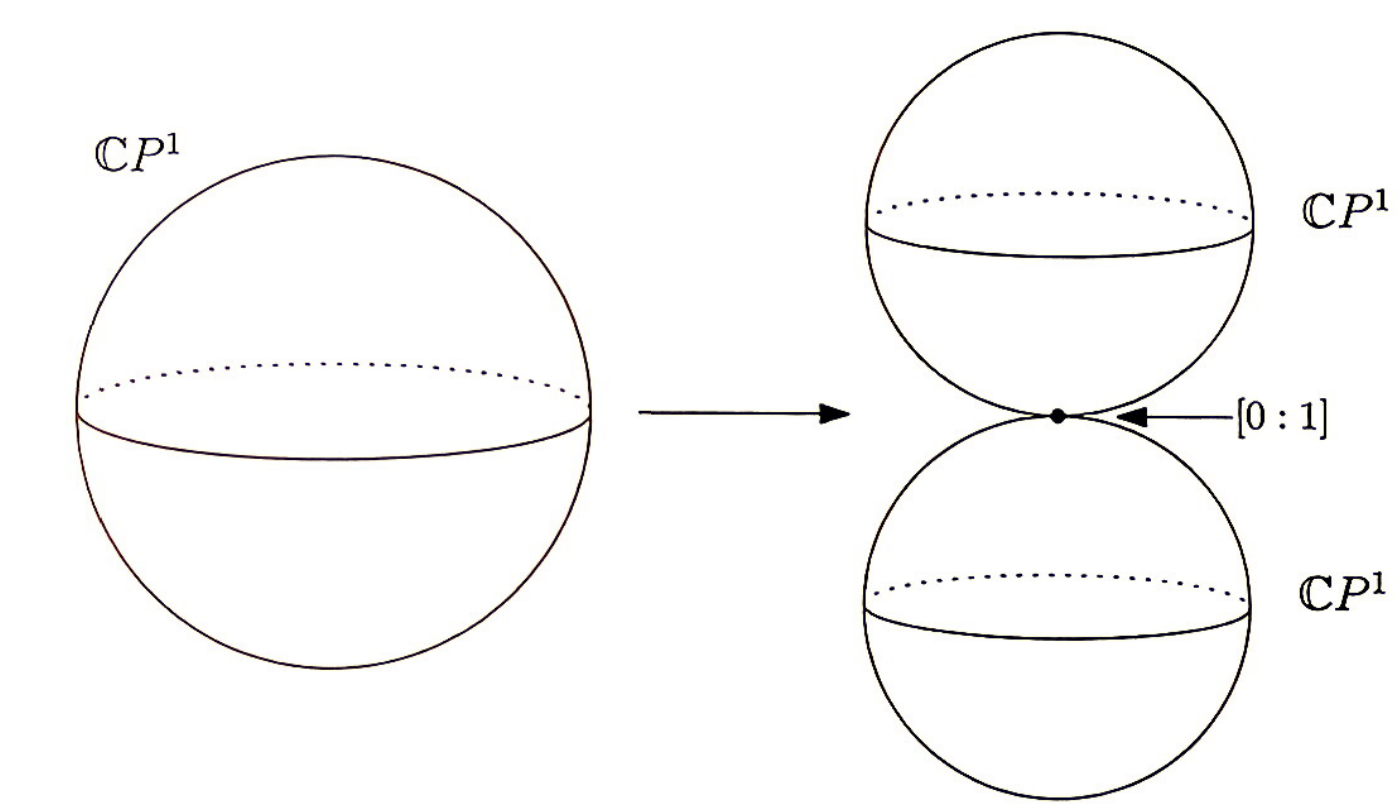
\includegraphics[width=0.52\linewidth]{figures/fig_p213_1.png}
  \caption*{图 8.1\quad $\CP^1$ 分裂为两份 $\CP^1$（原书 p.205, Figure 8.1）}
\end{figure}
% [Tutor Note: 易错预警——冒泡是紧性失败的典型机制：$S^2$ 上的能量在 $u_n$ 中向某点集中，重标度
%  后「挤出」一个新的 $J$-全纯球面。此例中 $\omega_{\mathrm{FS}}$ 在两份 $\CP^1$ 上的积分分别为
%  $1$ 与 $1$，而 $u_n$ 的类是 $[u_n(S^2)]=2L$（$L$ 为直线类），故能量守恒
%  $2=\omega_{\mathrm{FS}}(2L)=\omega_{\mathrm{FS}}(A_0)+\omega_{\mathrm{FS}}(A_1)$。注意
%  (8.16) 中的同构 $\CP^1\setminus\{[0:1]\}\cong\C$ 说明极限映射在冒泡点「丢掉」了信息——这正是
%  必须把极限对象推广为「树 + 稳定映射」的原因。详见 8.3 节后文与第 5 章注 5.4.5。]

% >>> p214
\begin{wexer}{8.3.1}
  设 $u_n\colon(S^2,j)\to(\CP^2,J_{\mathrm{std}})$ 是一列 $J$-全纯曲线，其中 $\CP^2$ 取坐标
  $[Z_0:Z_1:Z_2]$，$J_{\mathrm{std}}$ 是其标准复结构，$u_n$ 由 (8.15) 定义。

  如上面所讨论的，其极限像在 $n\to\infty$ 时记为 $A_0\cup A_1$，其中 $A_0=\{Z_0=0\}$、
  $A_1=\{Z_1=0\}$。证明：存在一个 $J_{\mathrm{std}}$-全纯映射 $v\colon\CP^1\to\CP^2$，它覆盖
  分支 $A_0$（但遗漏分支 $A_1$），且把 $[1:0]$ 映到 $[0:0:1]$。（提示：考虑 $u_n$ 的重新参数化
  $v_n([z_0:z_1]):=u_n([z_0:nz_1])$。）
\end{wexer}

由于例 8.3.1 所展示的冒泡现象，在研究全体 $J$-全纯曲线之集合时，必须纳入更多的曲线——即这些曲线
的定义域不必是单份 $(S^2,j)$。我们将在本节末回到这一点。可以想象，在更复杂的情形中，会有多份
$(S^2,j)$ 以相当杂乱的构型相粘。例如，图 8.2 的左图给出了一个例子。为简化作图，人们通常用一棵
树 $T$ 来表示这一团 Riemann 2-球面（见图 8.2 右图）。这里，$T$ 的每个顶点代表一个 Riemann
2-球面，每条边代表一个粘合点。

\begin{figure}[htbp]
  \centering
  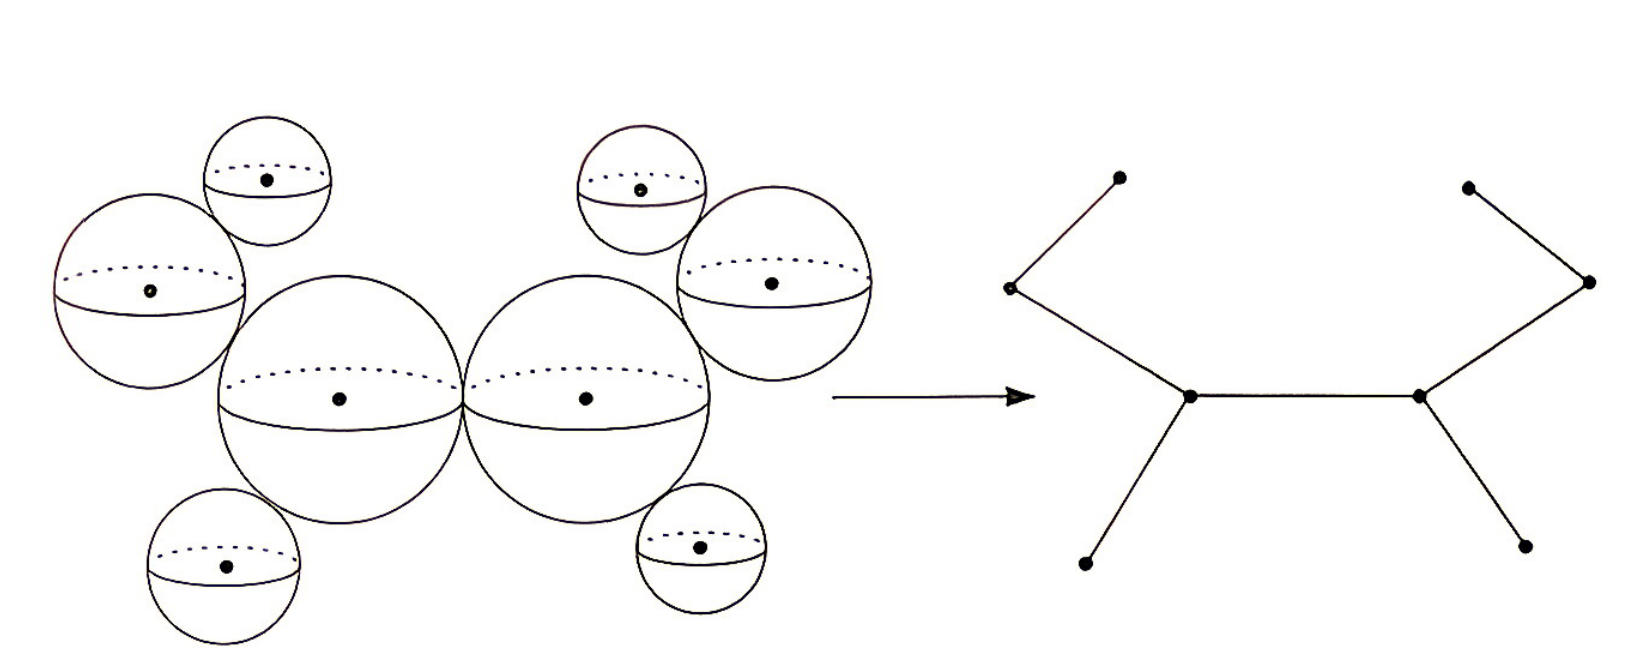
\includegraphics[width=0.86\linewidth]{figures/fig_p214_1.png}
  \caption*{图 8.2\quad 带树状构型的稳定映射（原书 p.206, Figure 8.2）}
\end{figure}

\textbf{多重覆盖曲线。} 研究曲线时的第二个问题是：曲线可能如 Riemann 曲面理论中那样是多重覆盖的
（见 [161] 第 III 章第 4 节），而同样的概念也适用于一般的 $J$-全纯曲线。

\begin{wdefn}{8.3.1}
  设 $u\colon(\Sigma_g,j)\to(M,J)$ 是一条 $J$-全纯曲线。若存在一条 $J$-全纯曲线
  $u'\colon(\Sigma_{g'},j)\to(M,J)$ 与一个全纯映射 $\varphi\colon\Sigma_g\to\Sigma_{g'}$，
  使得下述图表交换，则称 $u$ 是\textbf{多重覆盖的}（multiply covered）：
  \begin{equation}\tag{8.18}
  \begin{array}{ccc}
    (\Sigma_g,j) & \xrightarrow{\ u\ } & (M,J)\\[2pt]
    {\scriptstyle\varphi}\big\downarrow & \nearrow{\scriptstyle u'} & \\[2pt]
    (\Sigma_{g'},j) & &
  \end{array}
  \end{equation}
\end{wdefn}
% [Tutor Note: 易错预警——定义 8.3.1 照原文只要求 $\varphi$ 是全纯映射，未要求
%  $\deg(\varphi)\geqslant2$。但若允许 $\varphi$ 是同构（$\deg\varphi=1$），则任何曲线都能平凡地
%  「分解」成自己，多重覆盖的概念就失去意义；按惯例应补上 $\deg(\varphi)\geqslant2$（或等价地
%  要求 $u$ 与 $u'$ 不等价）。原文在此处的省略属常见简写，核对文献时请以「$\deg\varphi\geqslant2$」
%  为准；已记入 qsg/notes/review_ch08.md。]

% >>> p215
\begin{wthm}{8.3.1}（Riemann--Hurwitz 公式，[161] 中的定理 4.1.6）
  对紧可定向曲面之间的分支覆盖映射 $\varphi\colon\Sigma_g\to\Sigma_{g'}$，有
  \begin{equation}\tag{8.19}
    2g-2=\deg(\varphi)\cdot(2g'-2)+\sum_{p\in\Sigma_g}(e_p-1),
  \end{equation}
  其中 $e_p(\geqslant1)$ 表示点 $p\in\Sigma_g$ 的分支指数。
\end{wthm}

下面是定理 8.3.1 的一个容易的推论：若 $\Sigma_g=S^2$，即 $g=0$，则底曲面 $\Sigma_{g'}$（被覆盖者）
必须是 $S^2$；否则 (8.19) 的左端 $=-2<0\leqslant$ 右端，矛盾。然而，作为 $\Sigma_{g'}=S^2$ 的
多重覆盖，曲面 $\Sigma_g$ 可以有任意亏格 $g\geqslant0$。

\begin{wrem}{8.3.1}
  在某种程度上，这一拓扑障碍在本书中可能不那么有用，因为我们将只关心定义域为 $(S^2,j)$ 的
  $J$-全纯曲线。
\end{wrem}

引入辛结构的信息，即三元组 $(M,\omega,J)$，我们还可以对某条 $u'\colon(S^2,j)\to(M,\omega,J)$ 的
多重覆盖 $u$，考察其类 $A=[\operatorname{im}(u\colon S^2\to M)]\in H_2^S(M)$。于是
\begin{equation}\tag{8.20}
  B:=[\operatorname{im}(u'\colon S^2\to M)]=\frac{A}{\deg(\varphi)}\in H_2^S(M).
\end{equation}
取决于本章开头所介绍的背景辛流形 $(M,\omega)$ 的复杂性，关系式 (8.20) 可能是不可能成立的。下面是
一个例子。

\begin{wexam}{8.3.2}
  考虑定义 8.0.1 中半正辛流形的情形 (iii)，其中 $c_1(TM)$ 在 $H_2^S(M)$ 上的取值有很大的跳跃，
  间隔为 $4$（于是 $n\geqslant6$）。那么任何 $u$，只要其相伴的类 $A$ 满足 (8.20) 中的
  $c_1(TM)(A)=4$，就不可能是（任何 $u'$ 的）多重覆盖；否则，由于 $\deg(\varphi)\geqslant2$，
  我们知道 (8.20) 中的类 $B$ 满足 $c_1(TM)(B)=2$（当 $\deg(\varphi)=2$ 时）或
  $c_1(TM)(B)=1$（当 $\deg(\varphi)=4$ 时）。这样我们便得到矛盾，因为 $c_1(TM)$ 作用在
  $H_2^S(M)$ 中类 $A$ 与 $B$ 上的两个值之差为
  \[
    c_1(TM)(A)-c_1(TM)(B)=4-2=2\quad\text{或}\quad4-1=3,
  \]
  小于我们假设中的最小间隔 $4$。\hfill$\square$
\end{wexam}

若一个 Riemann 曲面不是分支覆盖的，则称它是\textbf{单的}（simple）。下述定义又是把这一概念直接
搬到 $J$-全纯曲线上。

% >>> p216
\begin{wdefn}{8.3.2}
  若 $J$-全纯曲线 $u\colon(\Sigma,j)\to(M,J)$ 不是定义 8.3.1 意义下的多重覆盖，则称它是
  \textbf{单的}（simple）。
\end{wdefn}

\begin{wrem}{8.3.2}
  若 $J$-全纯曲线 $u\colon(S^2,j)\to(M,J)$ 不是单的（即是多重覆盖的），则总存在一条单的
  $J$-全纯曲线 $u'\colon(S^2,j)\to(M,J)$，使得 $u$ 是 $u'$ 的多重覆盖。粗略地说，这是因为
  不能一直除以 $\deg\geqslant2$，故必须在有限步内停下来。停下来时，覆盖映射 $\varphi$ 的唯一可能
  情形是满足 $\deg(\varphi)=1$。回到公式 (8.19)，我们有 $\sum_{p\in\Sigma_g}(e_p-1)=0$，这
  意味着没有分支点，$\varphi$ 是 $S^2$ 上的全纯微分同胚，即一次重新参数化（见紧接其后的
  「重新参数化」小节）。类似的论证表明：本注第一句话的结论对定义域为 $(\Sigma_g,j)$（任意
  $g\geqslant0$）的任何多重覆盖 $J$-全纯曲线 $u$ 也成立。
\end{wrem}

一般地判定一条曲线是否单的并不显然。对 $J$-全纯曲线，借助某些分析结果，可以导出一个相当快的
（且局部的）判据来检验 $J$-全纯曲线是否单。

\whead{事实}{8.3.1}（[243] 中的命题 2.6）\quad 对 $J$-全纯曲线
$u\colon(\Sigma,j)\to(M,J)$，它是单的当且仅当存在 $z\in\Sigma$，使得
$\dd u(z)\colon T_z\Sigma\to T_{u(z)}M$ 是单射，且 $u^{-1}(u(z))=\{z\}$。

\textbf{重新参数化。} 研究映射 $u\colon(\Sigma_g,j)\to(M,J)$ 时的最后一个问题是重新参数化，
即作用在 $\Sigma_g$ 上的全纯微分同胚。我们的动机来自下述基本观察：对 $J$-全纯曲线
$u\colon(S^2,j)\to(M,J)$，若它如定义 8.3.2 那样是单的，则我们仍会有一个形如 (8.18) 的图表，
但唯一的可能性如下：
\begin{equation}\tag{8.21}
\begin{array}{ccc}
  (S^2,j) & \xrightarrow{\ u\ } & (M,J)\\[2pt]
  {\scriptstyle\varphi}\big\downarrow & \nearrow{\scriptstyle u'} & \\[2pt]
  (S^2,j) & &
\end{array}
\end{equation}
其中 $u'\colon(S^2,j)\to(M,J)$ 是某个 $J$-全纯映射，而
$\varphi\colon(S^2,j)\to(S^2,j)$ 是全纯微分同胚（或等价地，双全纯映射）（见注 8.3.2）。由于
$u=u'\circ\varphi$，我们有 $u'=u\circ\varphi^{-1}$，这意味着 $u'$ 可看作映射 $u$ 的一次重新
参数化。
% [Tutor Note: 原文疑误——(8.21) 之前的正文写「we will still have a diagram like (??)」，其中
%  (??) 是原书未解析的交叉引用，按上下文应为 (8.18)。译文按「形如 (8.18) 的图表」处理，已记入
%  qsg/notes/review_ch08.md。]

记 $\mathrm{Aut}(S^2)$ 为 $(S^2,j)$ 上全体双全纯映射构成的群。则一方面，从任何 $J$-全纯映射
$u$ 出发，通过前复合 $\varphi\in\mathrm{Aut}(S^2)$，我们将得到另一条 $J$-全纯曲线
$u\circ\varphi$；另一方面，一个众所周知的结果是
$\mathrm{Aut}(S^2)\cong\mathrm{PSL}(2,\C)$，它是一个维数为 $6$（在 $\R$ 上）的非紧群。
所有这些合起来表明：就 $J$-全纯曲线的计数而言，真正应当计数的对象是模去重新参数化后的
「类」，而非曲线本身。

% >>> p217
为更精确地描述这一点，让我们引入一些记号。记
\begin{equation}\tag{8.22}
  \mathcal{C}(M,J):=\bigl\{J\text{-全纯曲线 }u\colon(S^2,j)\to(M,J)\bigr\}.
\end{equation}
群 $\mathrm{PSL}(2,\C)$ 通过 $\varphi\cdot u:=u\circ\varphi$ 作用在集合
$\mathcal{C}(M,J)$ 上。于是我们将关心等价类之集 $\mathcal{C}(M,J)/\sim$，其中 $u\sim v$
当且仅当存在某个 $\varphi\in\mathrm{PSL}(2,\C)$ 使得 $v=\varphi\cdot u$。

\begin{wrem}{8.3.3}
  就 $\mathrm{PSL}(2,\C)$ 在 $\mathcal{C}(M,J)$ 上的群作用而言，人们会试图考察陪集与稳定化子
  之间的关系。不幸的是，对一般的 $u\in\mathcal{C}(M,J)$，稳定化子
  $\mathrm{PSL}(2,\C)_u$ 并不容易分析或描述。相反地，一旦考虑 (8.23) 中的加强版本，情形就大不
  相同（见注 8.3.4）。
\end{wrem}

这里还有 $J$-全纯曲线的另一个修改版本，它对稍后在 8.5 节引入的 Gromov--Witten 不变量的定义特别
有用。这里的映射 $u$ 除 $J$-全纯之外，还伴随其定义域 $(S^2,j)$ 上一个整数 $k\geqslant0$ 对应的
$k$ 元有序互异点组（有时这称为\textbf{带点 Riemann 球面}，pointed Riemann sphere）。换言之，
我们考虑如下元素：
\begin{equation}\tag{8.23}
  (u,(z_1,\cdots,z_k))\in\mathcal{C}(M,J)\times\bigl((S^2\times\cdots\times S^2)
    \setminus\Delta_k\bigr),
\end{equation}
其中 $\Delta_k$ 是 $k$ 份 $S^2\times\cdots\times S^2$ 的「大」对角线，使得
$(z_1,\cdots,z_k)$ 是 $k$ 元有序互异点组。再次地，重新参数化问题出现了，我们在 (8.23) 中定义
等价关系：$(u,(z_1,\cdots,z_k))\sim(v,(w_1,\cdots,w_k))$ 当且仅当存在某个
$\varphi\in\mathrm{PSL}(2,\C)$ 使得
\begin{equation}\tag{8.24}
  v=u\circ\varphi\qquad\text{且}\qquad w_i=\varphi(z_i)\quad(1\leqslant i\leqslant k).
\end{equation}
稍后我们将看到，(8.22) 中 $\mathcal{C}(M,J)$ 的基数（它通常是无穷的）在给 (8.23) 中的标记点
$(z_1,\cdots,z_k)$ 加上约束后会迅速降为有限的数。
% [Tutor Note: 术语依据——「marked point」译「标记点」，「pointed Riemann sphere」译「带点
%  Riemann 球面」；$\Delta_k$ 称为「大对角线」(big diagonal)，即存在 $i\ne j$ 使 $z_i=z_j$ 的
%  点组之集（与通常的对角线 $\{z_1=\cdots=z_k\}$ 不同，故加「大」字）。注意 (8.24) 的等价关系
%  必须同时作用在映射与标记点上，否则计数对象会把同一条曲线的不同标记方式重复计入。]

\begin{wrem}{8.3.4}
  （参看注 8.3.3）若 (8.23) 中 $k\geqslant3$，则由 (8.24) 定义的 $\mathrm{PSL}(2,\C)$ 在
  $\mathcal{C}(M,J)\times((S^2\times\cdots\times S^2)\setminus\Delta_k)$ 上的群作用，对任何
  $(u,(z_1,\cdots,z_k))$ 都有平凡的迷向群。确实，$(S^2,j)$ 上任何固定三个（或更多个）互异点的
  双全纯映射必为恒同映射。
\end{wrem}

\textbf{稳定映射的模空间。} 稳定映射的概念综合了前面三个小节的全部要素。它最早由 M. Kontsevich
在 [139] 中引入。

\begin{wdefn}{8.3.3}
  设 $(M,J)$ 是近复流形。\textbf{稳定映射}（stable map）由下述数据定义。
  % >>> p218
  \begin{enumerate}[label=(\roman*)]
    \item 其定义域（记作 $T$）是一个\textbf{树状构型}，由有限多个 Riemann 球面 $(S^2,j)$ 以某种
          方式相粘而成（粘合点通常称为\textbf{结点}，nodal point；这样的构型称为
          \textbf{结点曲线}，nodal curve）。这些 Riemann 球面构成顶点集 $v(T)$，粘合点构成边集
          $e(T)$。
    \item 在 $v(T)$ 的每个 $S^2$-分支上，映射 $u$ 都是 $J$-全纯映射。
    \item 若 $v(T)$ 中某个 $S^2$-分支上的限制是常值映射，则该分支上至少有三个互异标记点，
          其中包括 $e(T)$ 中的粘合点。
  \end{enumerate}
\end{wdefn}

给 $T$ 配上由 $v(T)$ 中每个 $S^2$-分支诱导的标准复结构。若稳定映射
$u\colon(T,j)\to(M,J)$ 在 $v(T)$ 的至少一个 $S^2$-分支上的限制按定义 8.3.1 是多重覆盖的，则称
$u$ 是\textbf{多重覆盖的}；否则称 $u$ 是\textbf{单的}。

\begin{wrem}{8.3.5}
  稳定映射 $u\colon(T,j)\to(M,J)$ 的重新参数化，由分别作用在 $v(T)$ 每个 $S^2$-分支上的重新
  参数化，再加上树 $T$ 自身的自同构带来的额外作用共同定义。
\end{wrem}
% [Tutor Note: 含糊点拨——定义 8.3.3 只写出「数据结构」而没有直接写出稳定性条件，稳定性条件藏在
%  第 (iii) 条里：常值分支必须至少带三个标记点（包括粘合点），其作用是让该分支上的自同构群有限。
%  这与代数几何中 Deligne--Mumford 稳定曲线（每个 $\mathbb{P}^1$ 分支上「特殊点」总数 $\ge3$）
%  是同一条件。原书对一般 $S^2$-分支不要求标记点数，是因为非平凡 $J$-全纯球面的自同构群本来
%  有限；只有在分支退化为常值时才有额外自由度，需要标记点钉住。]

下面我们考察 $J$-全纯曲线的各种模空间。其中有四个出现得相当频繁。固定一个辛流形 $(M,\omega)$ 与
一个与之相容的近复结构 $J$。重要的是，再固定一个类 $A\in H_2^S(M)$。来自类 $A$ 的约束正是这里
的模空间与 (8.22) 或 (8.23) 中的 $\mathcal{C}(M,J)$ 之间的本质差别。

(i) 这是可以写出的最简单的模空间。固定任意整数 $k\geqslant0$，记
\[
  \mathcal{M}^*_k(A,J):=\left\{
    \begin{array}{l}
      \text{单的 }J\text{-全纯曲线 }u\colon(S^2,j)\to(M,\omega,J)\\
      \text{带 }k\text{ 个标记点，且 }[u(S^2)]=A
    \end{array}\right\}\Big/\mathrm{PSL}(2,\C).
\]
特别地，$\mathcal{M}^*_k(A,J)$ 中的记号 $*$ 表示「单的」$J$-全纯曲线。由于重新参数化小节中
讨论的 $\mathrm{PSL}(2,\C)$ 群作用，$\mathcal{M}^*_k(A,J)$ 中的元素都是等价类。

(ii) 下面是由 (i) 加强而来的两个模空间。
\[
  \mathcal{M}_k(A,J):=\left\{
    \begin{array}{l}
      J\text{-全纯曲线 }u\colon(S^2,j)\to(M,\omega,J)\\
      \text{带 }k\text{ 个标记点，且 }[u(S^2)]=A
    \end{array}\right\}\Big/\mathrm{PSL}(2,\C)
\]
% >>> p219
及
\[
  \overline{\mathcal{M}^*_k(A,J)}:=\left\{
    \begin{array}{l}
      \text{单的稳定映射 }u\colon(T,j)\to(M,\omega,J)\\
      \text{带 }k\text{ 个标记点，且 }[u(T)]=A
    \end{array}\right\}\Big/G.
\]
这里，$\overline{\mathcal{M}^*_k(A,J)}$ 中的作用群 $G$ 就是注 8.3.5 所述的那个群，而
$[u(T)]=A$ 意指
\begin{equation}\tag{8.25}
  [u(T)]=\sum_{S^2\in v(T)}[u(S^2)]=A.
\end{equation}

\begin{wrem}{8.3.6}
  可以固定一棵树 $T$，并构造另一个模空间 $\mathcal{M}^*_{k,T}(A,J)$ 作为
  $\overline{\mathcal{M}^*_k(A,J)}$ 的子集。事实上，可以把 $\overline{\mathcal{M}^*_k(A,J)}$
  看作所有可能的树状构型 $T$ 对应的 $\mathcal{M}^*_{k,T}(A,J)$ 的并。
\end{wrem}

(iii) 正如人们可以预料的，这是最复杂的、由上面 (ii) 中各空间进一步加强而来的模空间：
\begin{equation}\tag{8.26}
  \overline{\mathcal{M}_k(A,J)}:=\left\{
    \begin{array}{l}
      \text{带 }k\text{ 个标记点且 }[u(T)]=A\\
      \text{的稳定映射 }u\colon(T,j)\to(M,\omega,J)
    \end{array}\right\}\Big/G.
\end{equation}
这里，群 $G$ 的作用与 $[u(T)]=A$ 的含义都与 (ii) 中 $\overline{\mathcal{M}^*_k(A,J)}$ 的情形
相同。唯一的差别是：$\overline{\mathcal{M}_k(A,J)}$ 中的稳定映射可以是多重覆盖的。

这四个模空间之间的关系可由下图说明：
\[
\begin{array}{ccc}
  \mathcal{M}^*_k(A,J) & \xrightarrow{\ c\ } & \mathcal{M}_k(A,J)\\[4pt]
  {\scriptstyle c}\big\downarrow & \searrow{\scriptstyle i}
    & \big\downarrow{\scriptstyle c}\\[4pt]
  \overline{\mathcal{M}^*_k(A,J)} & \xrightarrow{\ c\ }
    & \overline{\mathcal{M}_k(A,J)}
\end{array}
\]
其中 $i\colon\mathcal{M}^*_k(A,J)\to\overline{\mathcal{M}_k(A,J)}$ 是自然的包含映射。
% [Tutor Note: 易错预警——请核对图中四个空间与四个箭头的对应：横向箭头 $c$ 表示「取闭包/紧化」
%  的一步（把简单曲线换成简单稳定映射、把一般曲线换成稳定映射），纵向箭头 $c$ 表示「去掉单性
%  条件」，而斜箭头 $i$ 才是真正意义上的包含
%  $\mathcal{M}^*_k(A,J)\subset\overline{\mathcal{M}_k(A,J)}$。原文四个箭头都用了字母 $c$，
%  容易看混；另注意 $\mathcal{M}^*_k$ 与 $\mathcal{M}_k$ 上带横线的是紧化，不带横线的不紧。]

下述定理是这些模空间上最重要的结果之一。

\begin{wthm}{8.3.2}（Gromov [99]）
  设 $(M,\omega)$ 是辛流形，$J$ 是 $M$ 上 $\omega$-相容的近复结构，$A$ 是 $H_2^S(M)$（按 (8.4)
  定义）中的非零同调类。对上面 (i)、(ii)、(iii) 中所定义的模空间，存在
  $\mathcal{M}_k(A,J)$ 上的一个拓扑（称为 \textbf{Gromov 序列拓扑}，Gromov sequential
  topology），使得它的紧化恰为 $\overline{\mathcal{M}_k(A,J)}$，且
  $\mathcal{M}^*_k(A,J)$ 是 $\overline{\mathcal{M}_k(A,J)}$ 中的开稠子集。此外，对通有的
  $\omega$-相容近复结构 $J$，模空间 $\mathcal{M}^*_k(A,J)$ 具有（实）流形结构，且其（实）维数
  等于
  \begin{equation}\tag{8.27}
    \dim_\R\mathcal{M}^*_k(A,J)
      =\dim_\R M+2c_1(TM)(A)+2k-6.
  \end{equation}
\end{wthm}

更一般地，对注 8.3.6 中固定树状构型 $T$ 的模空间 $\mathcal{M}^*_{k,T}(A,J)$，若它（对通有的
$\omega$-相容 $J$）是（实）流形，则其（实）维数为
% >>> p220
\begin{equation}\tag{8.28}
  \dim_\R\mathcal{M}^*_{k,T}(A,J)
    =\dim_\R M+2c_1(TM)(A)+2k-6-2(\#e(T)),
\end{equation}
其中 $e(T)$ 表示 $T$ 的边集。
% [Tutor Note: 易错预警——(8.27) 中 $2k-6$ 的来历：$\mathrm{PSL}(2,\C)$ 在 $\R$ 上维数为 6，
%  而每个标记点贡献 2 个实参数，故 $\mathcal{M}^*_k$ 的维数比「未模去重新参数化」的维数少
%  $6-2k$。注意当 $k<3$ 时该维数可能为负，此时模空间（对通有 $J$）空集——这正是注 8.3.4
%  所要求的 $k\geqslant3$ 的几何来源。(8.28) 中再多减 $2\#e(T)$：每条边（结点）粘合时损失
%  $2$ 个实参数。]

\begin{wrem}{8.3.7}
  定理 8.3.2 中的公式 (8.27) 可视为公式 (8.28) 当树 $T$ 只是一个点时的特殊情形。
\end{wrem}

我们还记 $\mathrm{vir\text{-}dim}(\overline{\mathcal{M}_k(A,J)})$ 为 (8.27) 中算出的
$\dim_\R\mathcal{M}^*_k(A,J)$，无论 $\mathcal{M}^*_k(A,J)$ 是否具有流形结构。这里
$\mathrm{vir\text{-}dim}$ 称为模空间 $\overline{\mathcal{M}_k(A,J)}$ 的\textbf{虚拟维数}
（virtual dimension）。此外，为简化措辞，在谈论上述模空间的元素时我们常常省略「等价类」一词。

下面是标准的例子。

\begin{wexam}{8.3.3}
  取 $(M,\omega,J)=(\CP^2,\omega_{\mathrm{FS}},J_{\mathrm{std}})$，其中
  $\omega_{\mathrm{FS}}$ 是 Fubini--Study 辛结构，$J_{\mathrm{std}}$ 是 $\CP^2$ 上的标准复
  结构。记 $L$ 为 $H_2(\CP^2;\Z)$ 的生成元，它由标准直线 $\CP^1\subset\CP^2$ 代表。固定
  $A=2L\in H_2^S(\CP^2)=H_2(\CP^2;\Z)$。让我们研究
  $\overline{\mathcal{M}_k(A,J)}=\overline{\mathcal{M}_0(2L,J_{\mathrm{std}})}$。该模空间中
  会出现若干个层。

  例如，$\overline{\mathcal{M}_k(A,J)}=\overline{\mathcal{M}_0(2L,J_{\mathrm{std}})}$ 包含
  一个（很大的）子集：由 $(S^2,j)\simeq(\CP^1,J_{\mathrm{std}})$ 到 $\CP^2$ 的全纯映射的像
  所构成的（等价类）——即 $\CP^2$ 中的\textbf{光滑圆锥曲线}（smooth conic），因为这些映射的
  次数为 $2$。用 $[X:Y:Z]$ 表示 $\CP^2$ 的坐标，则光滑圆锥曲线由
  \[
    aX^2+bY^2+cZ^2+dXY+eXZ+fYZ=0
  \]
  定义。该表达式在 $\C$ 中有 $6$ 个系数，但自由的有 $5$ 个（差一个整体伸缩），因此该集合的维数
  $\dim_\C=5$（即 $\dim_\R=10$）。事实上，这些光滑圆锥曲线之集正是模空间
  $\mathcal{M}^*_0(2L,J_{\mathrm{std}})$。由定理 8.3.2，$\mathcal{M}^*_0(2L,J_{\mathrm{std}})$
  是 $\overline{\mathcal{M}_0(2L,J_{\mathrm{std}})}$ 的开稠子集，而公式 (8.27) 算出
  $\dim_\R=4+2\cdot(2\cdot(2+1))+2\cdot0-6=10$。

  除这些光滑圆锥曲线外，还可以有退化情形。例如，类 $A=2L$ 可以来自（复）直线的双重覆盖
  （次数为一的曲线）。注意由定理 8.3.1，若映射
  $u\colon(S^2,j)\to(\CP^2,J_{\mathrm{std}})$ 是双重覆盖的，则其底映射也是从 $(S^2,j)$ 出发的
  映射，并且
  \[
    2\cdot0-2=2\cdot(2\cdot0-2)+\sum_{\text{分支点 }p}(e(p)-1),
  \]
  这蕴涵有两个分支点。这些合起来给出了所有此类双重覆盖之集的复 $4$ 维自由度。同样地，例 8.3.1
  所精确刻画的正是：类 $A=2L$ 也可以来自结点曲线，即两份 $(S^2,j)$
\end{wexam}

% >>> p221
相粘。于是每份 $S^2\simeq\CP^1$ 分别有复 $1$ 维自由度，这蕴涵所有此类结点曲线之集的维数为
$2$。对这种结点曲线情形，我们也可以从定理 8.3.2 的公式 (8.28) 得到同样的结果，其中树状构型
$T$ 如图 8.3 所示、$\#e(T)=2$。此时相应的模空间具有（实）维数
$4+2\cdot(2\cdot(2+1))+2\cdot0-6-2=8$。当然，还有进一步的退化情形，其相应的模空间维数更低
（余维更高）。\hfill$\square$

\begin{figure}[htbp]
  \centering
  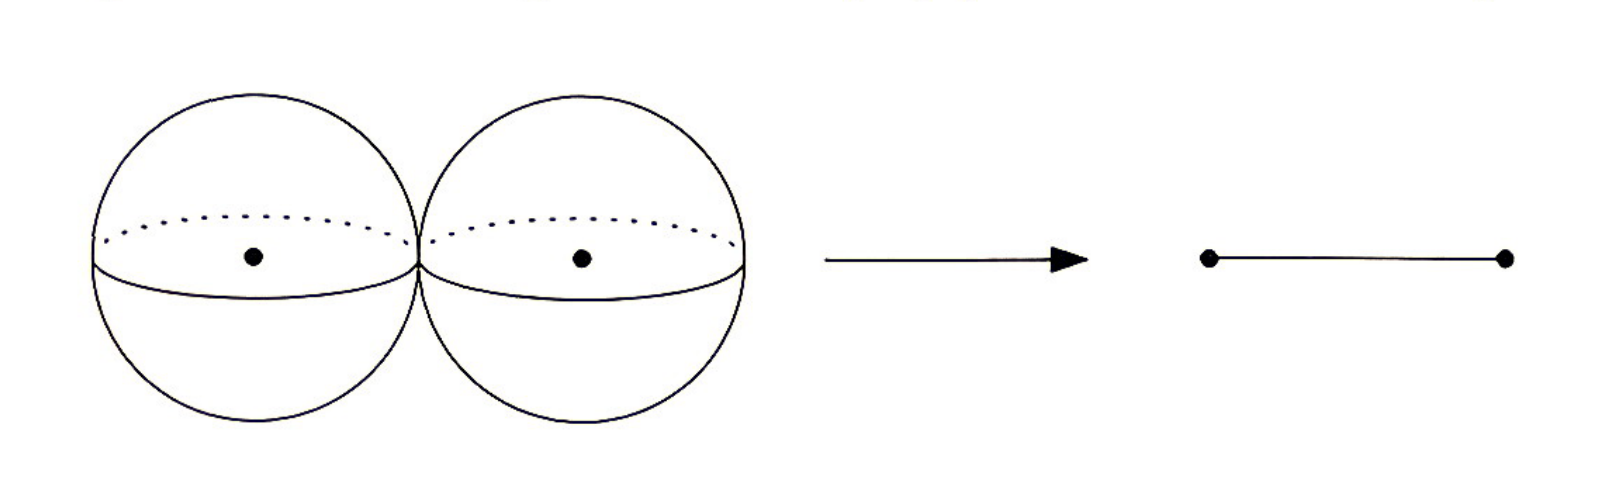
\includegraphics[width=0.66\linewidth]{figures/fig_p221_1.png}
  \caption*{图 8.3\quad 两份 $S^2$ 的构型（原书 p.213, Figure 8.3）}
\end{figure}

例 8.3.3 是下述分层结构的一个具体例子：
\begin{equation*}
\begin{aligned}
  \overline{\mathcal{M}_k(A,J)}
    &=\mathcal{M}^*_k(A,J)\cup
      \left(\begin{array}{l}
        \text{来自多重覆盖或结点曲线的}\\
        \text{严格低维（开）层}
      \end{array}\right)\\
    &=\mathcal{M}^*_k(A,J)\cup
      \Bigl(\bigcup_T\mathcal{M}^*_{k,T}(A,J)\cup(\text{多重覆盖})\Bigr).
\end{aligned}
\end{equation*}
人们通常用图 8.4 来说明这样的分层。粗略地说，由定理 8.3.2 中的 (8.28)，树状构型 $T$ 越复杂
（即 $\#e(T)$ 越大），注 8.3.6 中相应的模空间 $\mathcal{M}^*_{k,T}(A,J)$ 的维数就越低。

\begin{figure}[htbp]
  \centering
  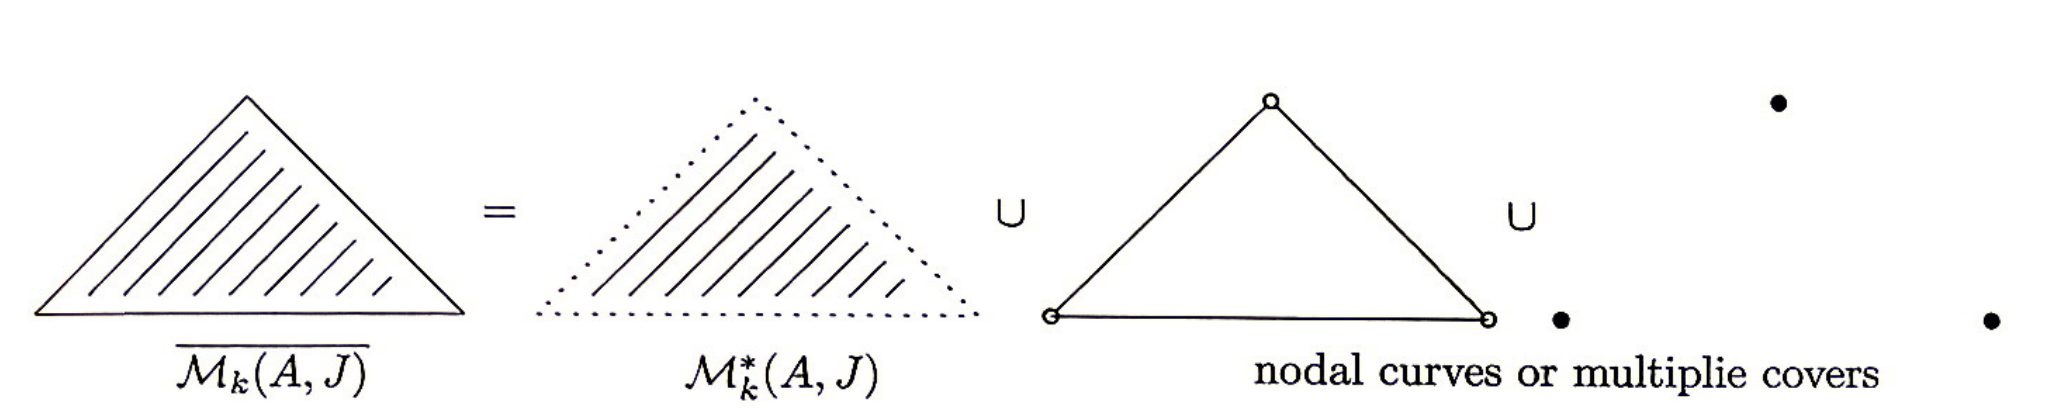
\includegraphics[width=0.86\linewidth]{figures/fig_p221_2.png}
  \caption*{图 8.4\quad $\overline{\mathcal{M}_k(A,J)}$ 的分层（原书 p.213, Figure 8.4）}
\end{figure}
% [Tutor Note: 含糊点拨——这一分层公式是 Gromov--Witten 理论的技术核心：紧化空间
%  $\overline{\mathcal{M}_k(A,J)}$ 是若干个（可能有奇点的）低维层的并，最高维的开层是单曲线
%  的模空间 $\mathcal{M}^*_k(A,J)$。计数 GW 不变量时只取最高维层的「虚拟基本类」，但分层结构
%  决定了粘合公式（与量子乘积的结合性/WDVV 方程直接相关，见 8.7 节）。图 8.4 中左端三角代表
%  整个 $\overline{\mathcal{M}_k}$，右端用「结点曲线或多重覆盖」标出补集。]

\begin{wexer}{8.3.2}
  对辛流形 $(\CP^1,\omega_{\mathrm{FS}},J_{\mathrm{std}})$，仿照例 8.3.3 研究模空间
  $\overline{\mathcal{M}_0(L,J_{\mathrm{std}})}$，其中 $L\in H_2^S(\CP^1;\Z)(=H_2(\CP^1;\Z))$
  是由 $\CP^1$ 中标准直线代表的类。
\end{wexer}
